\documentclass[professionalfont]{beamer}

\usepackage[T1]{fontenc}
\usepackage{amsmath}
\usepackage{graphicx}
\graphicspath{{figures/}}
\usepackage{tikz}
\usepackage{algorithm}
\usepackage[noend]{algpseudocode}
\usepackage{color}
\usepackage[export]{adjustbox}

\DeclareMathOperator*{\argmin}{argmin}

% usage: \tikzpic{<x percent>}{<y percent>}{<image size>}{<image name>}
\newcommand*{\tikzpic}[4]{%
\begin{tikzpicture}[remember picture,overlay]
\node at (current page.south west) [xshift=#1\paperwidth,yshift=#2\paperheight] {\includegraphics[width=#3\linewidth]{#4}};
\end{tikzpicture}%
}

\title[Importance Sampling based transfer in RL]{\textbf{\\Importance Sampling based \\ transfer in RL}}
\author[A. Sessa]{\textbf{\emph{Andrea Sessa}}\\
{\small{Mat. 850082}}
\vspace{2mm}
{\small \href{}{\nolinkurl{}}}\\
 \small{Supervisor: Prof. \emph{Marcello Restelli}} \\
 \small{Cosupervisor: Dott. \emph{Matteo Pirotta}}}
\date{}

\usetheme{POLIMI}

\expandafter\def\expandafter\insertshorttitle\expandafter{\insertshorttitle\hfill\insertframenumber\,/\,\inserttotalframenumber}

\begin{document}

  \begin{frame}[plain]
    \titlepage
  \end{frame}

  \section{Introduction}
    \begin{frame}
    \frametitle{Introduction}
      \textcolor{red}{\textbf{Motivation}}: solving a task in Reinforcement Learning, in general, is not easy: \textbf{a lot} of experience (interactions with the environment)
      is needed. In many real-world situation (e.g. robotics) this can be a problem.\newline

      Many times previous experience in tasks similar to the target one is available.\newline

      \textcolor{blue}{\textbf{Goal}}: reuse the past experience to speed-up the learning performance in the target task
      avoiding at the same time the \textbf{negative transfer} problem.
    \end{frame}

  \section{RL}
    \begin{frame}
	  \frametitle{Reinforcement Learning (RL)}
      A task in the context of RL is formalized as a \textcolor{blue}{\textbf{Markov Decision Process}} (MDP). \newline
      A MDP is defined a tuple, $<\mathcal{S}, \mathcal{A}, \mathcal{P}, \mathcal{R}, \gamma>$, where:
      \begin{itemize}
        \item $\mathcal{S}$ is the state space.
        \item $\mathcal{A}$ is the action space.
        \item $\mathcal{P}: \mathcal{S} \times \mathcal{A} \rightarrow \Pi(\mathcal{S})$ is \textbf{transition} function.
        \item $\mathcal{R}: \mathcal{S} \times \mathcal{A} \rightarrow \Pi(\mathbb{R})$ is the \textbf{reward} function.
        \item $\gamma \in [0,1]$ is the discount factor for the MDP.
      \end{itemize}
      The goal is learn an optimal (greedy) \textcolor{red}{\emph{policy}}:
      \begin{equation*}
        \pi^{*}(s) = arg\max_{a \in \mathcal{A}} Q^{*}(s,a)
      \end{equation*}
      where $Q^{*}(s,a)$ (optimal Q-function) accounts for the discounted expected reward.
    \end{frame}

  \section{Batch RL}
	   \begin{frame}
  	 \frametitle{Batch Reinforcement Learning}
     In the rest of this presentation we will assume the context of \textbf{Batch RL}:\newline

     An \textbf{experience sample} is defined as a tuple $(s,a,s',r)$. \newline

     \pause
     Then the learning procedure is divided into two distinct phases:
     \begin{itemize}
       \item \textcolor{red}{\textbf{Sampling Phase}}: Samples are collected from the MDP and stored.
       \item \textcolor{blue}{\textbf{Learning Phase}}: The samples collected in the previous phase are
        used to learn a policy $\pi$ over the MDP.
     \end{itemize}
     The separation between the two phases gives us some advantages in the transfer procedure.
   \end{frame}


  \section{Transfer Learning}
	   \begin{frame}
  	 \frametitle{Transfer Learning}
     We denote using $T$ the target task.\newline
     We denote by $\{ S_{i} \}_{i=1}^{N_{s}}$ the set of source tasks.\newline

     We focus on the transfer of experience \textcolor{violet}{\textbf{samples}} from ${S_i}$ to $T$.\newline
     \pause
     The transfer is achieved by associating a weight $w \geq 0$ to each sample:
     \begin{itemize}
       \item $w \approx 0$ indicates a sample that should \textcolor{red}{\textbf{not}} be transferred to $T$.
       \item $w > 0$ indicates a sample that should be transferred to $T$.
     \end{itemize}
     \vspace{.7cm}
     Every sample in $T$ has $w = 1$.
  	\end{frame}

  \section{Importance Sampling}
     \begin{frame}
  	 \frametitle{Importance Sampling}
      Weights are calculated using the idea of \textcolor{red}{\textbf{Importance Sampling}}:\newline

      For each sample $(s,a,s',r)$ we consider two weights $w_r$ and $w_s$ associated
      to the reward and transition described by the sample.\newline
      \pause

      Using the theory of Importance Sampling the definition of the weights is:
      \begin{equation*}
        w_s = \frac{\mathcal{P}_{\textcolor{red}{T}}(s'|s,a)}{\mathcal{P}_{\textcolor{violet}{S}}(s'|s,a)} \quad
        w_r = \frac{\mathcal{R}_{\textcolor{red}{T}}(r|s,a)}{\mathcal{R}_{\textcolor{violet}{S}}(r|s,a)}
      \end{equation*}
      And then taking $w = w_{r}w_{s}$.\newline

      The estimations is \textcolor{blue}{\textbf{unbiased}} but the variance could be very high (even infinite in some situation).
  	\end{frame}

   \section{Estimating1}
      \begin{frame}
    	\frametitle{Estimating the weights - 1}
      In practice the model of rewards and transition are not known.\newline

      We use a pair of \textcolor{orange}{\textbf{Gaussian Process regressor}} (\textcolor{red}{Gaussian} assumption) for each task (target included).\newline
      Under these conditions the weight are distributed according to an unknown distribution.\newline
      \pause

      We are able to prove the following result:
      \begin{equation*}
        \mathbb{E}[\tilde{w}_{x}(\tilde{\mu}_{T}, \tilde{\mu}_{S})] =
        \begin{cases}
          \frac{\sigma^{2}}{\sigma^{2} - \sigma^{2}_{GP,S}} \frac{\mathcal{N}(x; \mu_{GP,T}, \sigma^{2} + \sigma^{2}_{GP,T})}{\mathcal{N}(x; \mu_{GP,T}, \textcolor{red}{\sigma^{2} - \sigma^{2}_{GP,S}})} \quad \sigma^{2}_{GP,S} < \sigma^{2} \\
          \infty \quad Otherwise
        \end{cases}
      \end{equation*}
      where $x$ can be either $r$ or $s'$.
    	\end{frame}

    \section{Estimating2}
       \begin{frame}
       \frametitle{Estimating the weights - 2}
       The previous equation could be used but may lead to very high weights
       when $\sigma^{2}$ approaches $\sigma^{2}_{GP,S}$ and the algorithm
       may need to discard the sample when $\sigma^{2} > \sigma^{2}_{GP,S}$.\newline

       \pause
       A possible \textcolor{blue}{\textbf{heuristics}} may be proposed as:
       \begin{equation*}
         \tilde{w}(x) = \frac{\mathcal{N}(x; \mu_{GP,T}, \sigma^{2}+\sigma^{2}_{GP,T})}{\mathcal{N}(x; \mu_{GP,S}, \sigma^{2} + \sigma^{2}_{GP,S})}
       \end{equation*}
       which still converges to the ideal weights when the GP are perfectly accurate.
       \end{frame}

    \section{Comparison}
      \begin{frame}
      \frametitle{Comparing different estimations}
        \begin{figure}
          \includegraphics[scale=0.5]{images/comparison.eps}
          \caption{}
          \label{}
        \end{figure}
      \end{frame}
    \section{Comparison2}
      \begin{frame}
      \frametitle{Comparing different estimations}
        \begin{figure}
          \includegraphics[scale=0.5]{images/comparison2.eps}
          \caption{}
          \label{}
        \end{figure}
      \end{frame}


    \section{(W)FQI}
      \begin{frame}
      \frametitle{Using the weights - (W)FQI}
        We apply our weight estimation procedure to a well known Batch RL
        algorithm: \textcolor{red}{\textbf{Fitted Q-Iteration (FQI)}} \newline
        \pause
        The main idea of FQI is to use the samples collected in conjunction
        with a \textcolor{orange}{\textbf{regression} algorithm} to obtain at each iteration
        an increasingly better estimation of the Q-function. \newline
        \begin{equation*}
          \hat{Q}^{k+1} = arg\min_{f \in \mathcal{F}} \frac{1}{N_{t}} \sum_{i=1}^{N_t} ||f(s_{i}, a_{i}) - \mathcal{T}\hat{Q}^{k}||^{2}
        \end{equation*}
        \pause

        Using a \textcolor{blue}{\textbf{weighted} regression} algorithm permits to exploit the
        capability of FQI adding the possibility to transfer samples across
        multiple tasks.\newline
        \pause
        Given a sample $(s,a,s',r)$:
        \begin{equation*}
          \hat{Q}^{k+1} = arg\min_{f \in \mathcal{F}} \frac{1}{N_{t}\textcolor{red}{+N_{s}}} \sum_{i=1}^{N_{t}\textcolor{red}{+N_{s}}} \textcolor{red}{w_{i}}||f(s_{i}, a_{i}) - \mathcal{T}\hat{Q}^{k}||^{2}
        \end{equation*}
      \end{frame}

    \section{Experiments1}
      \begin{frame}
      \frametitle{Experiments - Puddle World}

      \begin{columns}
       \column{0.62
       \linewidth}
        \includegraphics[scale=0.4,left]{images/puddle.eps}

       \column{0.5\linewidth}
        \begin{itemize}
          \item \textcolor{red}{\textbf{Continuous}} state space
          \item \textcolor{red}{\textbf{Discrete}} action space
          \item Gaussian reward/transition model
        \end{itemize}
      \end{columns}

      \end{frame}

    \section{Experiments1}
      \begin{frame}
      \frametitle{Experiments - Sources and Target tasks}
      \begin{figure}
        \includegraphics[scale=0.55]{images/global.eps}
      \end{figure}
      \end{frame}

    \section{Experiments3}
      \begin{frame}
      \frametitle{Experiments - Puddle World - Ideal Weights}
        \begin{figure}
          \includegraphics[scale=0.5]{images/WFQIPerf_ID.eps}
          \label{}
        \end{figure}
      \end{frame}

    \section{Experiments4}
      \begin{frame}
      \frametitle{Experiments - Puddle World - Estimated Weights}
        \begin{figure}
          \includegraphics[scale=0.5]{images/WFQIPerf.eps}
          \label{}
        \end{figure}
      \end{frame}

      \section{Experiments2}
        \begin{frame}
        \frametitle{Experiments - Acrobot}

        \begin{columns}
         \column{0.42
         \linewidth}
          \includegraphics[scale=0.25,left]{images/acrobot.png}

         \column{0.5\linewidth}
          \begin{itemize}
            \item \textcolor{red}{\textbf{Continuous}} state space
            \item \textcolor{red}{\textbf{Discrete}} action space
            \item \textcolor{blue}{\textbf{Non}}-gaussian reward/transition model
          \end{itemize}
        \end{columns}
        \end{frame}

    \section{Experiments5}
      \begin{frame}
      \frametitle{Experiments - Acrobot - Estimated Weights}
        \begin{figure}
          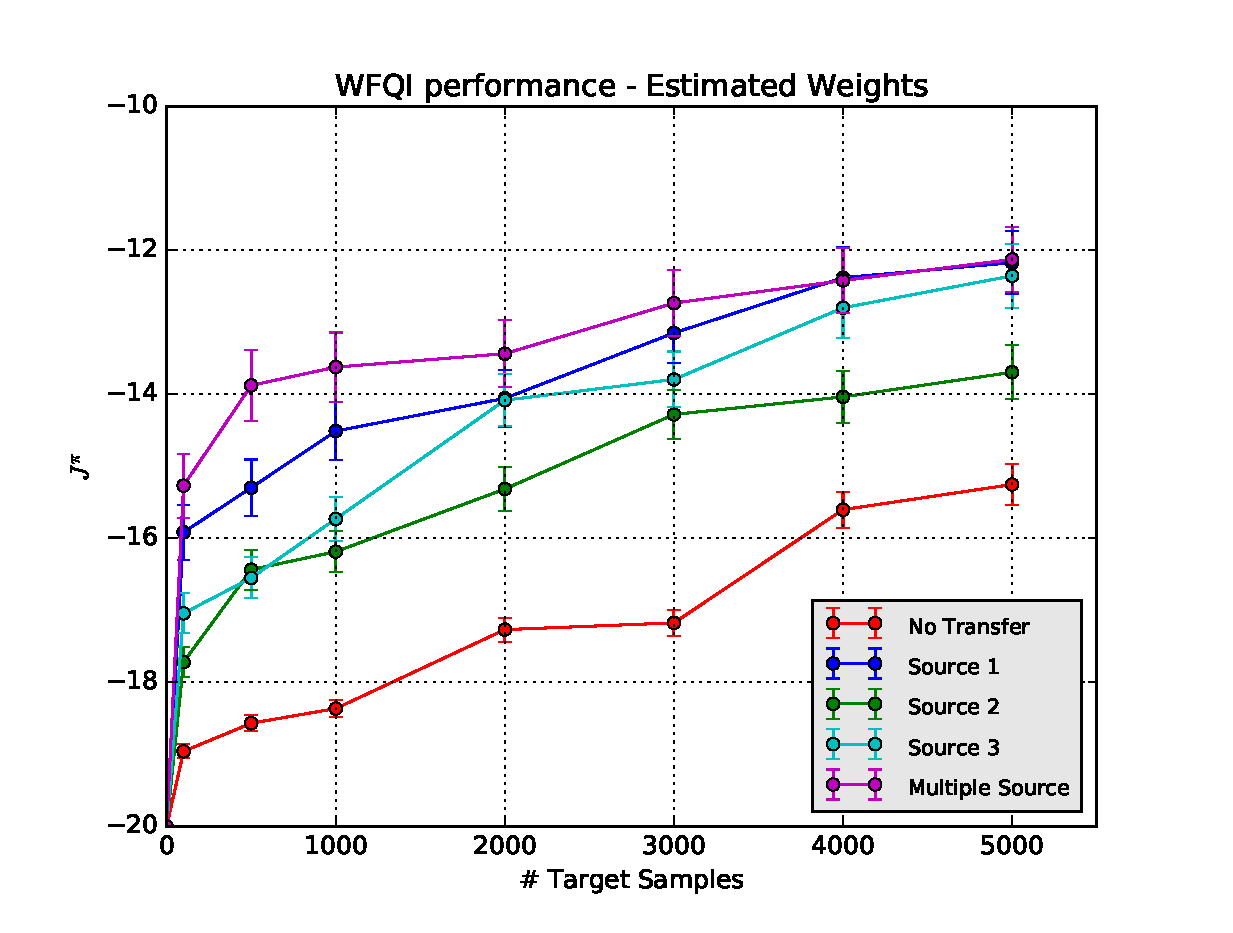
\includegraphics[scale=0.5]{images/WFQIPerf_acro.eps}
          \label{}
        \end{figure}
      \end{frame}

    \section{Conclusions}
    \begin{frame}
      \frametitle{Conclusions - Future Developments}
      We have developed a transfer learning approach with a strong \textcolor{red}{\textbf{theoretical}}
      background (not shown).\newline

      \textcolor{blue}{\textbf{Empirical}} result over different environments have shown the effectiveness of such approach.\newline

      Possible future developments:
      \begin{itemize}
        \item More effective weights selection procedure
        \item Application to more challenging environments
      \end{itemize}
    \end{frame}

    \section{Additional}
    \begin{frame}
      \pause
      \frametitle{Additional - The Algorithm}
      \begin{figure}
        \includegraphics[scale=0.45]{images/wfqi.png}
      \end{figure}
    \end{frame}

\end{document}
